\documentclass[a4paper,12pt,titlepage,oneside,openany]{book}
\usepackage[top=3cm,bottom=3cm]{geometry}
\usepackage[italian]{babel}
\usepackage[utf8]{inputenc}
\usepackage{amsmath,amssymb,amsfonts,amsthm,graphicx,mathrsfs,braket,float}
\usepackage[hidelinks]{hyperref}
\usepackage{bytefield}
\usepackage{multirow}
\usepackage{url}
\setcounter{secnumdepth}{4} 
\setcounter{tocdepth}{3}
\linespread{1.6}
\graphicspath{ {./Images/} }

\begin{document}
	\clearpage
	\thispagestyle{empty}
	\begin{figure}
		\centering
		\vspace*{-2cm}	
\includegraphics[scale=0.6]{logounict.png}
		\label{fig:logounict}
	\end{figure}
	
	
	\centerline{{\LARGE UNIVERSIT\`{A} DEGLI STUDI DI CATANIA}}
	\centerline{DIPARTIMENTO DI MATEMATICA E INFORMATICA} \centerline{CORSO DI LAUREA MAGISTRALE IN INFORMATICA}
	\centerline{\rule{16cm}{0.2mm}}\vspace*{2cm}
	\centerline{\LARGE{Distributed Dictionary Attack}}
	\centerline{\LARGE{}}
	\centerline{\rule{1cm}{0.2mm}}\medskip
	\centerline{RELAZIONE}
	\centerline{\rule{1cm}{0.2mm}}
	\vspace*{1.19cm}
	\begin{minipage}[t]{0.47\textwidth}
		\raggedright{
			\makebox[3cm][l]{Studenti}\par
			\makebox[3cm][l]{Pietro Biondi}\par
			\makebox[3cm][l]{Giuseppe Parasiliti}\par
		}\vspace*{0.5cm}
	\end{minipage}
	\begin{minipage}[t]{0.47\textwidth}
		\raggedleft{
			\makebox[3cm][l]
			{Professore}\par
			\makebox[3cm][l]
			{Emiliano Tramontana}\par} \vspace*{0.5cm}
	\end{minipage}
	
	\centerline{\rule{16cm}{0.2mm}} 
	\centerline{ANNO ACCADEMICO 2017/2018}
	\newpage
	\thispagestyle{empty}
	\tableofcontents
	\thispagestyle{empty}
	\newpage
\chapter{Introduzione}
Al giorno d'oggi si sente sempre più parlare di account compromessi. Spesso la causa di tutto ciò è la poca attenzione che l'utente mette nella scelta di password banali o comunque poco robuste e facilmente indovinabili. L'autenticazione basata su conoscenza è vulnerabile sotto diversi attacchi tra cui quelli a forza bruta e dizionario.
Il progetto ha come obbiettivo quello di effettuare un attacco a dizionario in ambiente distribuito, dove coesistono diversi attaccanti con lo scopo di violare il sistema target ottenendo migliori risultati soprattutto dal punto di vista della velocità.
\section{Tassonomia di attacchi alle password}
\subsection{Attacco a forza bruta}
In informatica il metodo "forza bruta" è noto anche come ricerca esaustiva della soluzione. Esso è un algoritmo di risoluzione di un problema dato che consiste nel verificare tutte le soluzioni teoricamente possibili fino a che si trova quella effettivamente corretta. Nell'ambito della sicurezza informatica, questo metodo si utilizza soprattutto per trovare la password di accesso a un sistema. Utilizzando una parola italiana di 8 caratteri come password, la sua robustezza è data dal numero totale di parole italiane di 8 caratteri. È quindi palese l'importanza di utilizzare password molto lunghe.
\subsection{Attacco a dizionario}
Un'altra tipologia di attacco per violare la password di un sistema può essere quello di sferrare un attacco a dizionario, che consiste nel provare le password contenute in un determinato dizionario. L'efficacia di un attacco a dizionario è direttamente proporzionale alla dimensione del dizionario stesso, in altre parole più è grande il glossario delle parole più è alta la probabilità di indovinare la password del sistema. L'efficacia di un attacco a dizionario può essere notevolmente ridotta limitando il numero massimo di tentativi di autenticazione che possono essere effettuati sul sistema e bloccando anche i tentativi che superano una certa soglia di esiti negativi. Generalmente, tre tentativi sono considerati sufficienti per permettere ad un utente legittimo di correggere i propri errori di battitura e accedere correttamente al sistema. Superata questa soglia, l'utente potrebbe essere malintenzionato.
\section{Traccia dei contenuti}
La relazione è strutturata come segue:
\begin{itemize}
	\item[]\textbf{Capitolo 2 } in questo capitolo vengono spiegati tutti gli strumenti utilizzati per lo sviluppo del progetto.
	\item[]\textbf{Capitolo 3 } verranno affrontante in dettaglio l'implementazione del server.
	\item[]\textbf{Capitolo 4 } sarà spiegato in dettaglio l'implementazione della classe Attaccante.
\end{itemize}

\chapter{Strumenti utilizzati}
Per questo progetto sono stati utilizzati diversi strumenti e tecnologie. Tutto il progetto è stato sviluppato con il linguaggio di programmazione Java ed inoltre è stato utilizzato AspectJ. AspectJ\cite{aspectj} è un'estensione di Java per aggiungere a Java stesso i cosiddetti aspetti. È uno dei modi utilizzati per avvalersi dell'Aspect Oriented Programming. La programmazione orientata agli aspetti è un paradigma di programmazione basato sulla creazione di entità software - denominate aspetti - che sovrintendono alle interazioni fra oggetti finalizzate ad eseguire un compito comune. Il vantaggio rispetto alla tradizionale Programmazione orientata agli oggetti consiste nel non dover implementare separatamente in ciascuna classe il codice necessario ad eseguire questo compito comune. Inoltre, per la stesura del codice è stato utilizzato Eclipse\cite{eclipse} un Integrated Development Environment(IDE).\\
L'intera parte server-side è stata implementata con la tecnologia delle servlet. La comunicazione tra gli attaccanti avviene attraverso RabbitMQ\cite{rabbitmq}, esso è un message-oriented middleware. Il server RabbitMQ è scritto in Erlang e si basa sul framework Open Telecom Platform(OTP) per la gestione del clustering e del failover. Le librerie client per interfacciarsi a questo broker sono disponibili per diversi linguaggi tra cui Java.
\chapter{Sviluppo del server}
Per lo sviluppo del server è stata utilizzata la tecnologia delle Servlet\cite{servlet}. Per fare ciò è necessario un contenitore web che supporti la tecnologia Servlet, per questo motivo è necessario configurare un server Apache Tomcat. Eclipse mette a disposizione un wizard che guida lo sviluppatore nella configurazione totale del server web Apache Tomcat.
\section{Sviluppo LoginServlet}
Nel momento in cui il server riceve una richiesta di tipo POST, esso invocherà il metodo \textit{doPost} [\ref{fig:dopost}]. 
Tale metodo recupera l'username e la password ed assegna un cookie al client che ha inviato la richiesta. Successivamente inserisce il client all'interno di una struttura dati che gestisce il controllo d'accesso al sistema.\\
Una funzione principale per il corretto funzionamento del server è \textit{unBan}[\ref{fig:unban}]. Tale metodo controlla se il client, identificato attraverso il suo cookie, è stato bannato. In caso affermativo si controlla se è il momento di rimuovere il ban, questo controllo viene effettuato sul numero di tentativi e sulla differenza di tempo trascorsa tra il momento del ban e il momento corrente.
Come si può notare dalla [\ref{fig:unban}], all'interno del server vi è un sistema di ban incrementale direttamente  proporzionale al numero di tentativi effettuati. Il metodo unBan può ritornare tre valori:
\begin{itemize}
	\item[-] Valore 1: Indica che il client ha aspettato il tempo necessario e potrà essere sbloccato.
	\item[-] Valore 2: Indica che il client non ha ancora terminato il suo tempo di blocco.
	\item[-] Valore 3: Indica che il client non è bloccato.
\end{itemize}
\begin{figure}[H]
	\centering
	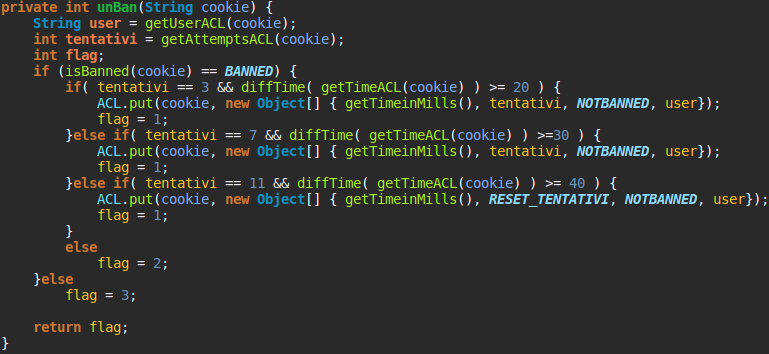
\includegraphics[scale=0.5]{unban.png}
	\caption{Funzione unban}
	\label{fig:unban}
\end{figure}
In base al valore restituito dalla funzione \textit{unBan}, il server restituisce al client tre tipologie di stato HTTP differenti. Nello specifico:
\begin{itemize}
	\item[-] Stato 270: Tale valore indica al client che è momentaneamente bloccato.
	\item[-] Stato 271: Esso indica al client che ha ancora dei tentativi a disposizione.
	\item[-] Stato 200: In caso di corretto login, il server restituirà al client tale valore.
\end{itemize}
\begin{figure}[H]
	\centering
	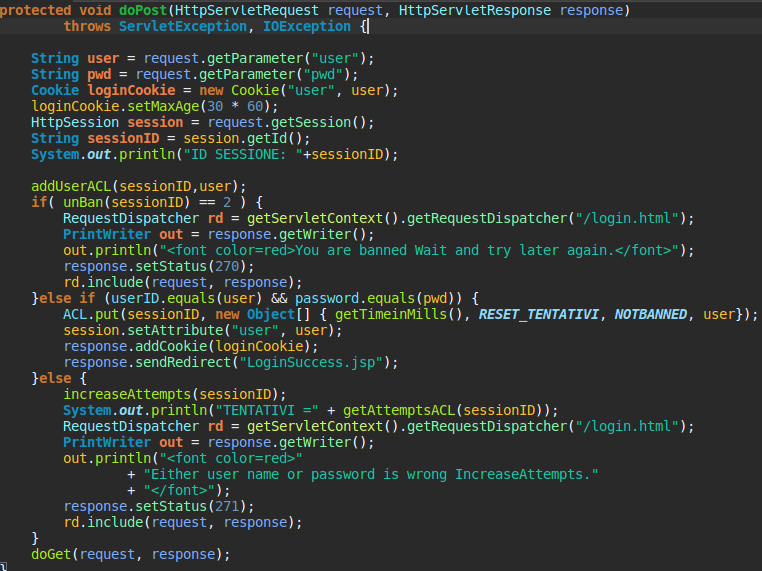
\includegraphics[scale=0.5]{dopost.png}
	\caption{Funzione doPost}
	\label{fig:dopost}
\end{figure}
\section{Aspect LogServer}
Nella figura sottostante, è implementato un pointcut che verrà eseguito nel momento in cui viene lanciato il metodo addUserACL. Tale pointcut stamperà l'ID (cookie) dell'utente che ha provato a connettersi.
\begin{figure}[H]
	\centering
	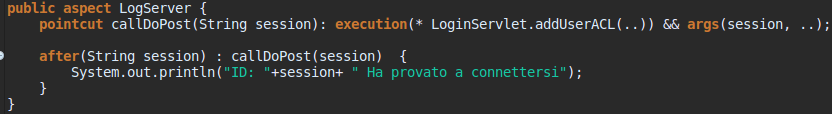
\includegraphics[scale=0.5]{logserver.png}
	\caption{Aspect logserver}
	\label{fig:logserver}
\end{figure}

\newpage
Nella figura [\ref{fig:jconsoleserver}] si può notare l'effetto del pointcut sopracitato, sulla console di Eclipse.
\begin{figure}[H]
	\centering
	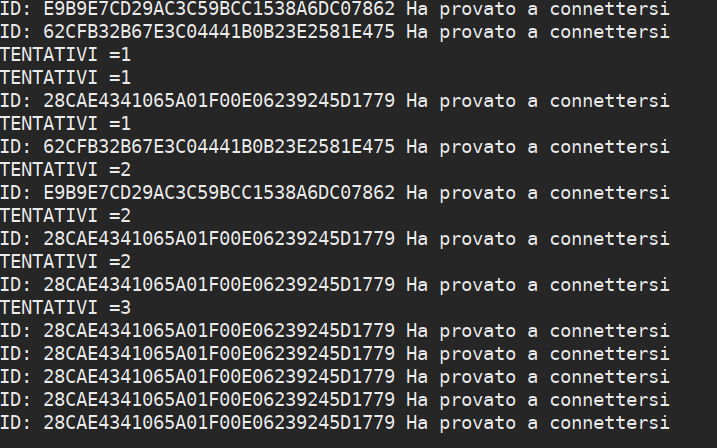
\includegraphics[scale=0.6]{jconsoleserver.png}
	\caption{Output pointcut server}
	\label{fig:jconsoleserver}
\end{figure}


\chapter{Implementazione classe Attacker}
In questo capitolo viene spiega l'implementazione della classe Attacker, che si occuperà di trovare la password per violare il sistema. Le funzioni principali utilizzate all'interno della classe sono: \textit{run}, \textit{sendMessage}, \textit{receivedMessage}.
\section{Funzione run}
Una volta invocata questa funzione, il client setta i parametri fondamentali per poter attaccare il sistema. Inizialmente, legge da un file il dizionario contenente tutte le password da provare. Successivamente, attraverso una richiesta GET al server, il client estrae le informazioni essenziali dal form che gli permetterà di costruire la richiesta POST in maniera corretta. Dopo di che verranno scelte le prime tre password con indice random che saranno inviate al server.
\begin{figure}[H]
	\centering
	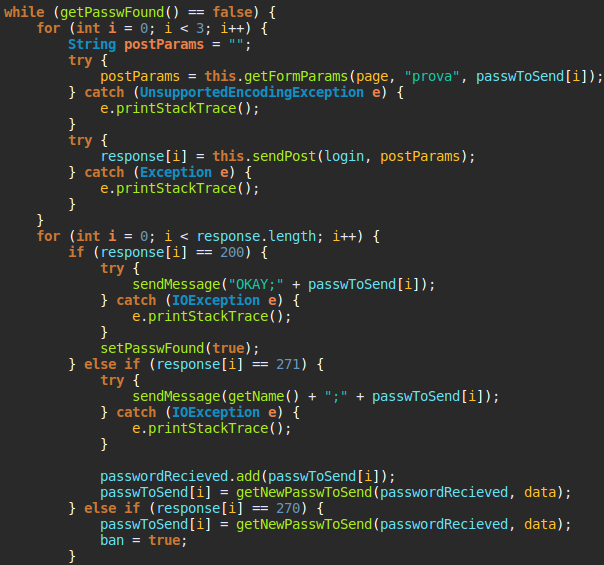
\includegraphics[scale=0.6]{run1.png}
	\caption{Funzione Run}
	\label{fig:run1}
\end{figure}
\noindent
Nella figura \ref{fig:run1} vengono costruiti tutti i parametri che successivamente verranno inviati al server attraverso la funzione \textit{sendPost}. Un esempio di questi parametri è:
\begin{itemize}
	\centering \item []“user=prova\&pwd=prova”
\end{itemize}
\noindent
Tale funzione restituirà, all'interno di un array(response), i valori dello status http che il server ha restituito per quella coppia username-password. Ogni risposta, all'interno dell'array response, verrà gestita con il costrutto “if annidato” che eseguirà differenti istruzioni a seconda del valore della risposta.
\begin{itemize}
	\item Se il valore della response è pari a \textit{200}: l'attaccante ha trovato la password e comunicherà a tutti gli altri attaccanti tale informazione.
	\item Se il valore della response è pari a \textit{271}: l'attaccante ha ancora a disposizione dei tentativi, invierà la password errata agli altri attaccanti per informarli di non utilizzarla.
	\item Se il valore della response è pari a \textit{270}: l'attaccante entrerà nello stato di ban. Quando l'attaccante è bloccato, entra in una fase di attesa che potrà finire in due casi: quando un altro attaccante ha trovato la password oppure allo scadere del tempo di ban.
\end{itemize}
Tutto il procedimento descritto dalla figura \ref{fig:run1} avviene fino a quando la password non verrà trovata.
\section{Funzione sendMessage}
La funzione descritta nella figura \ref{fig:sendMessage} permette di inviare la password in broadcast a tutti gli altri attaccanti. Questo avviene grazie alla funzione \textit{basicPublish} messa a disposizione dal middleware RabbitMQ.
\begin{figure}[H]
	\centering
	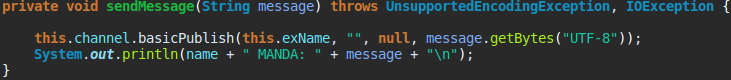
\includegraphics[scale=0.5]{sendMessage.png}
	\caption{Funzione sendMessage}
	\label{fig:sendMessage}
\end{figure}
\section{Funzione receivedMessage}
La funzione receivedMessage crea una classe anonima di tipo Consumer che effettuerà un Override del metodo \textit{handleDelivery}. Attraverso l'esecuzione della funzione\textit{channel.basicConsume} diremo al server RabbitMQ che la coda “queueName” dovrà essere utilizzata da quel “consumer”. Ciò è dovuto grazie alla callback handleDelivery che permette l'esecuzione del programma e non appena un messaggio viene inserito nella coda, il server Rabbit avviserà il client della presenza del nuovo messaggio. Una volta che il client consuma la coda esegue le istruzioni all'interno del metodo handleDelivery.
\begin{figure}[H]
	\centering
	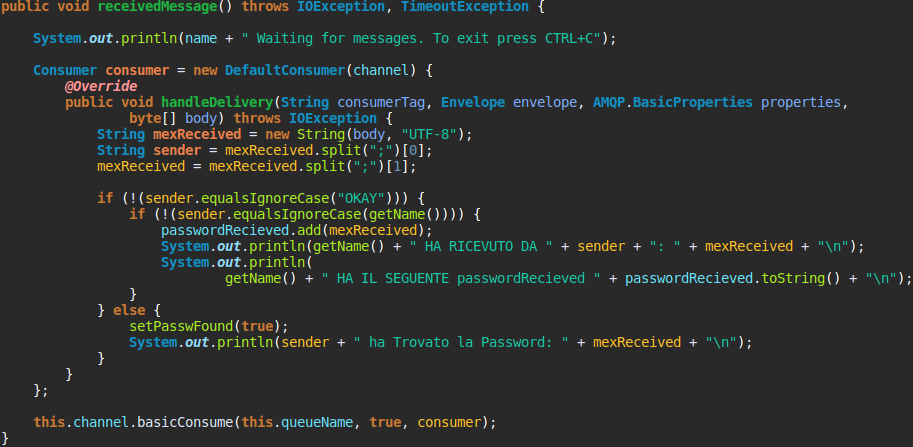
\includegraphics[scale=0.4]{receivedMessage.png}
	\caption{Funzione receivedMessage}
	\label{fig:receivedMessage}
\end{figure}
\section{Pointcut LogAttacker}
Nella figura sottostante, è implementato un pointcut che verrà eseguito nel momento in cui viene lanciato il metodo sendPost. Tale pointcut è diviso in due fasi differenti (before - after). Questo pointcut stamperà nella console: i parametri post che invierà al server e la risposta ricevuta da quest'ultimo.
\begin{figure}[H]
	\centering
	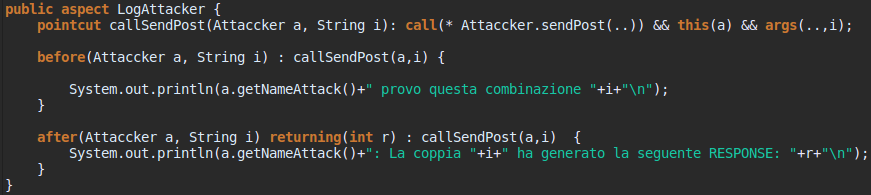
\includegraphics[scale=0.4]{logattacker.png}
	\caption{Pointcut logattacker}
	\label{fig:logattacker}
\end{figure}
\newpage
Nella figura sottostante si notare tutte le stampe eseguite dall'aspetto LogAttacker.
\begin{figure}[H]
	\centering
	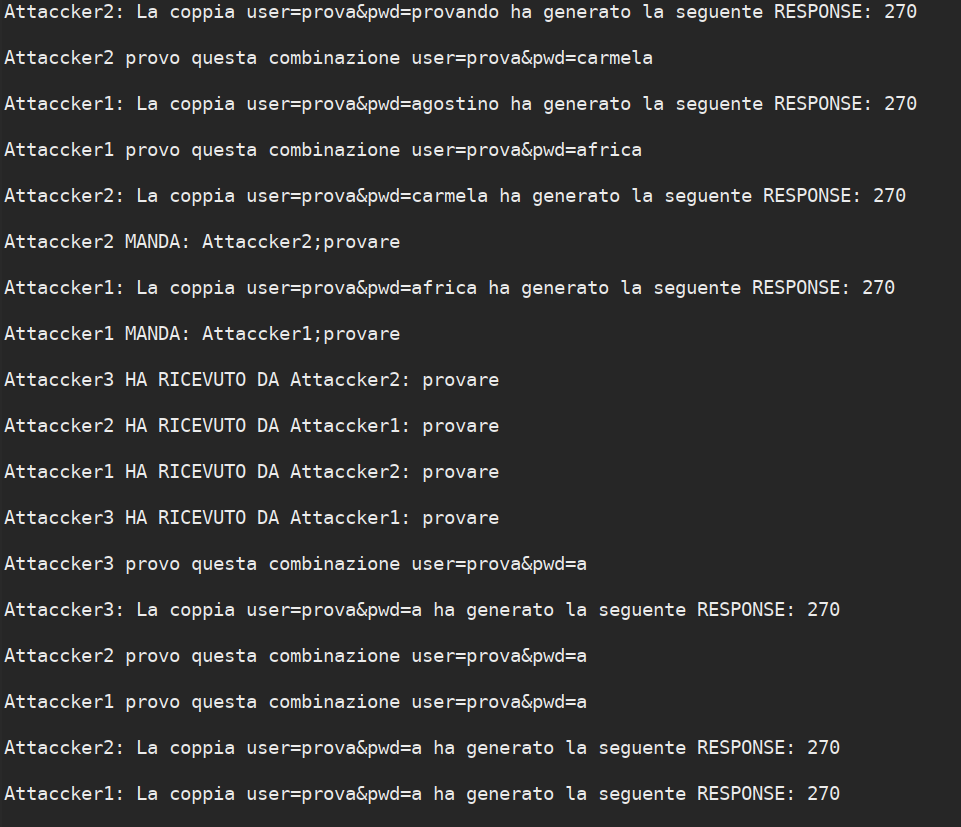
\includegraphics[scale=0.4]{jconsoleclient.png}
	\caption{Pointcut print console}
	\label{fig:jconsoleclient}
\end{figure}






\bibliographystyle{splncs}
\bibliography{biblio}
\end{document}